\chapter{Evaluatie van resource allocatieschema's}
\label{chap:evaluation}

In dit hoofdstuk wordt de eigenlijke Proof-of-Concept besproken en geëvalueerd. Met behulp van de testomgeving, beschreven in Hoofdstuk~\ref{sec:environment} en de monitor tools, uitgelegd in Hoofdstuk~\ref{chap:monitoring} is de hele evaluatie uitgevoerd.

De opbouw van dit hoofdstuk is als volgt. Eerst wordt er uitgelegd hoe de FaaFo-applicatie werklast kan genereren op één of meerdere worker-instanties. Vervolgens wordt een korte hypothese beschreven met het verwachte resultaat van de werking van Round Robin. Nadien wordt een test uitgevoerd met Rally om te bekijken of het schema naar behoren werkt op high-level niveau om af te sluiten met een stress-test, die wordt gemonitord en besproken.

\section{De schaalbare FaaFo-applicatie}
\label{sec:scalable_faafo}

Zoals besproken in Sectie~\ref{sec:faafo} is de FaaFo-applicatie uitermate geschikt om een stress-test uit te voeren op de drie gebruikte hypervisors met de RoundRobinScheduler ingeplugd in Nova. Na het activeren van de OpenStack stack kan er via de FaaFo-controller een commando worden ingegeven die voor voldoende werklast zal zorgen. De OpenStack-Orchestration en -Telemetry services laten dan alarmen afgaan bij een hoge werklast waardoor er extra worker-instanties aangemaakt worden. Zoals beschreven in de template in Sectie~\ref{sec:faafo_template} kunnen er maximum zeven worker-instanties tegelijkertijd actief zijn.

Op de OpenStack controller-node, jerico-03, kan dankzij de security group instellingen en de gebruikte sleutel (de key\textunderscore name parameter) een SSH-verbinding gelegd worden met de FaaFo-controller. Van hieruit kunnen er dan verschillende taken gestart worden als ook het weergeven van de huidige taken. De FaaFo-applicatie is zo gemaakt dat deze met volgende simpele commando's kan werken:

\begin{code}
\begin{minted}[breaklines]{bash}
$ faafo create --width 5555 --height 5555 --tasks 3
$ faafo list
\end{minted}
\caption{Starten van drie FaaFo-taken}
\end{code}

Het eerste commando zal 3 taken creëren die elk een fractaal moeten berekenen van de meegegeven hoogte en breedte. Deze drie taken komen dan terecht in de queue op FaaFo-controller waarna de FaaFo-workers een taak van de queue halen en deze uitvoeren. Het berekenen van een fractaal vergt veel CPU-verbruik en hierdoor zal het \textit{cpu\textunderscore alarm\textunderscore high}-alarm getriggerd worden. De OpenStack Orchestration-services, Heat, zullen hierop reageren door extra FaaFo-workers aan te maken.

Het tweede commando geeft een overzicht weer van de berekende en nog te berekenen fractalen, telkens met hun afmetingen en hun grootte op de harde schijf. Is de grootte nog nul, dan betekent dit dat het fractaal nog berekend moet worden, of dat er een FaaFo-worker mee bezig is

\section{Hypothese}

Round Robin is een contextloos algoritme, het weet niets af van de hosts hun capaciteiten. Bijgevolg wordt er verwacht dat de Rally-test een gunstig resultaat zal afleveren omdat deze test ook zonder context wordt uitgevoerd. Het gewoon starten en stoppen van instanties zonder generatie van werklast is ideaal voor een Round Robin schema en bijgevolg zullen alle instanties gelijkmatig verdeeld worden over de verschillende hosts.

In het geval van de schaalbare FaaFo-applicatie kunnen de nadelen van een Round Robin schema wel eens zichtbaar worden. De Orchestration-services van OpenStack verwijderen immers een willekeurige host bij een laag-cpu-alarm. Indien er nadien terug instanties bijkomen door een hoog-cpu-alarm, kan het zijn dat een host meer instanties bevat dan andere waardoor de werklast niet gelijk verdeeld zal worden.  In welke mate dit nadelig is, zal de test zelf moeten aantonen.

\section{Evaluatie met Rally}

De evaluatie met Rally gebeurt met dezelfde template zoals beschreven in Sectie~\ref{sec:rally}. Het enige verschil met de test die daar is uitgevoerd, is de gebruikte Nova-scheduler. De resultaten van de test zijn te zien in Figuur~\ref{fig:evaluation_rally}. De bovenste grafiek is de uitvoer van Rally zelf, gelijkaardig aan het resultaat uit Sectie~\ref{sec:rally}, de onderste grafiek is de uitvoer van de zelf ontwikkelde monitorapplicatie beschreven in Sectie~\ref{sec:monitor_tool}.

Zoals verwacht in de hypothese wordt de Rally-test beëindigd zonder fouten. Dit komt omdat de instanties steeds gelijkmatig worden verdeeld over de drie hosts. Dit is ook te zien in de Figuur~\ref{fig:evaluation_rally2} waarbij geen enkele host meer dan 2 instanties tegelijkertijd bezit. Verrassend aan het resultaat is dat de RoundRobin-scheduler er duidelijk langer over doet om alles te starten en te stoppen vergeleken met Figuur~\ref{fig:rally-test1} en Figuur~\ref{fig:rally-test2}. Doordat tegelijkertijd de nodejs-agent op de hosts data aan het verzamelen was, kan dit een mogelijke verklaring zijn voor de iets langere duurtijd.

Uit deze test kunnen volgende besluiten genomen worden. Omdat deze test contextloos is (er werd nergens werklast gegenereerd), werkt een RoundRobin-scheduler naar behoren. De werklast op de host jerico-03 is wel een pak groter dan die op de andere hosts. Een mogelijke verklaring hiervoor is het feit dat jerico-03 zowel de OpenStack-controller is en dus de andere hosts moet aansturen alsook zelf instanties moet hosten. Daarom is het aan te raden om een OpenStack-controller geen dienst te laten doen als hypervisor, zodat de werklast beter verdeeld kan worden.

\begin{figure}
	\centering
	\subcaptionbox{Uitvoer van Rally \label{fig:evaluation_rally1}}{%
		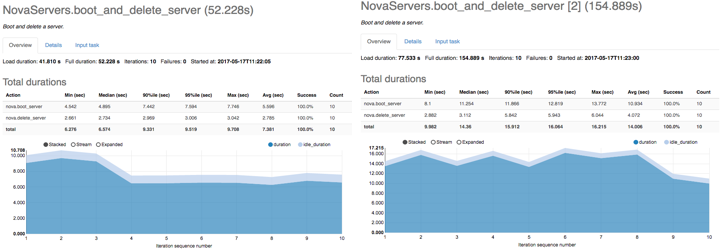
\includegraphics[width=1.00\textwidth]{Dia3}%
	}\par\medskip
	\subcaptionbox{Uitvoer van de monitorapplicatie \label{fig:evaluation_rally2}}{%
		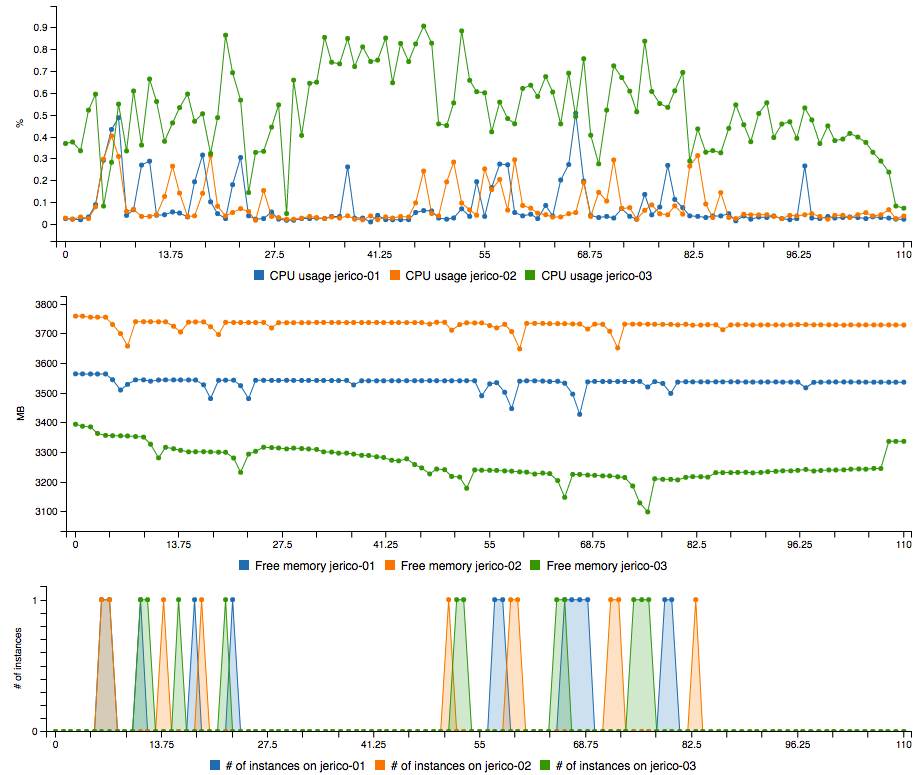
\includegraphics[width=1.00\textwidth]{rally_evaluation}%
	}
	\caption{Evaluatie met Rally - Resultaten}
	\label{fig:evaluation_rally}
\end{figure}

\section{Evaluatie met de FaaFo-applicatie}
\begin{figure}
	\centering
	\captionsetup{justification=centering}
	\begin{subfigure}{\textwidth}
		\centering
		\centerline{
			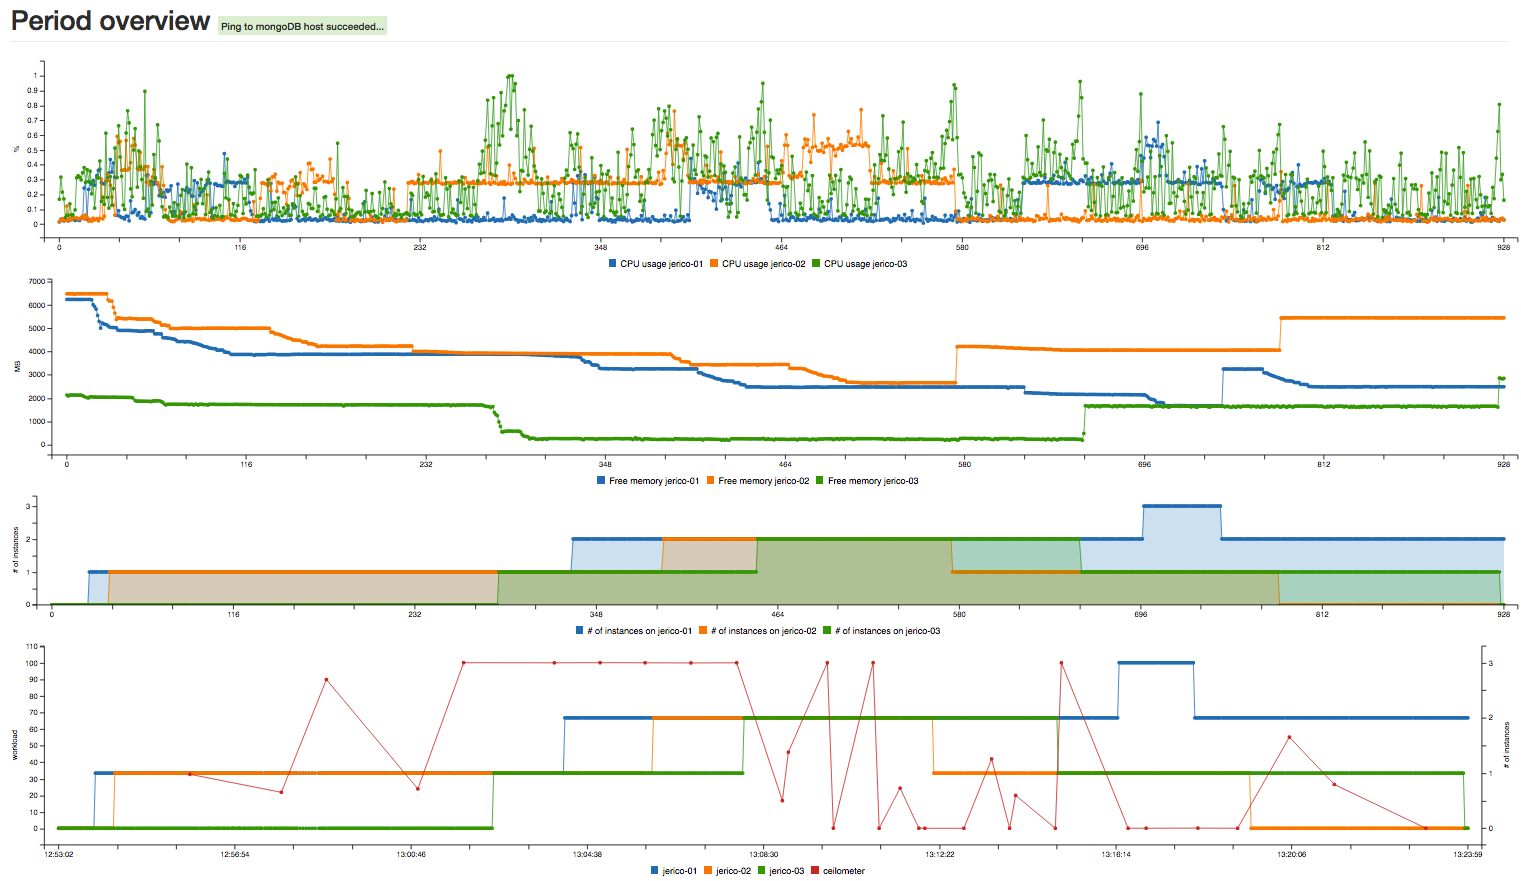
\includegraphics[width=\textwidth]{faafo_evaluation}
		}
	\end{subfigure}
	\caption{Resultaat van de stress-test met de FaaFo-applicatie}
	\label{fig:evaluation_faafo}
\end{figure}

Het Round Robin schema wordt ook getest met de schaalbare FaaFo-applicatie. De gemeten resultaten met de nodejs-agent bedekken de hele procedure, vanaf het creëren van de stack tot en met het voltooien van het \textit{faafo create}-commando en deze worden weergegeven in Figuur~\ref{fig:evaluation_faafo}.

Ook hier komen de resultaten goed overeen met de verwachte hypothese. De instanties worden in het begin evenredig verdeeld over de verschillende hosts. Ongeveer halverwege de resultaten zijn er enkele metingen met een laag cpu-gebruik, waardoor enkele worker-instanties verwijderd worden. Nadien worden terug hoge waarden gemeten van het cpu-gebruik waardoor nieuwe worker-instanties worden gestart. Deze nieuwe worker-instanties worden geplaatst op de eerstvolgende host in de rij van het Round Robin schema, zonder dat deze rekening houdt met de verwijderde instanties. Hierdoor zijn de instanties naar het einde van de test toe niet meer evenredig verdeeld en dat is ook zichtbaar in de derde en vierde grafiek.

Net zoals bij de Rally-test is de werklast op de OpenStack-controller groter dan bij de andere hosts. Ook de hoeveelheid vrij geheugen is beperkt op de OpenStack-controller in vergelijking met de andere hosts. In een worst-case scenario kan het zijn dat de instanties verwijderd worden op alle hosts met uitzondering van jerico-03, waardoor de hoeveelheid vrij geheugen op deze host te laag is om nog een nieuwe instantie te hosten. Indien de volgende nieuwe instantie dan net op jerico-03 gehost wordt, zorgt dit voor ernstige gevolgen zoals bijvoorbeeld het uitvallen van jerico-03 en dus de gehele OpenStack-omgeving.


\section{Resultaat van de evaluaties}

Een Round Robin schema is simpel en werkt naar behoren in de meeste gevallen. Het grootste nadeel is de contextloze eigenschap van dit schema waardoor er mogelijks problemen optreden bij een tekort aan fysieke resources. De gestelde hypothese voorafgaand aan de verschillende evaluaties is zeer aansluitend aan de verkregen resultaten mits het toevoegen van enkele bijkomende conclusies.

Door het hele proces te overlopen, vanaf het opzetten van de testomgeving tot de verschillende evaluaties, werd de Proof-of-Concept aangetoond. Het grootste deel van de gebruikte configuratie en code kan herbruikt worden bij andere allocatieschema's. Enkel het nieuwe schema moet worden geschreven in Python met de nodige overerving van de Nova-filters. Na die aanpassing is het mogelijk om het gehele evaluatieproces opnieuw te overlopen om zo de resultaten te bekomen, die nodig zijn voor de evaluatie van het nieuwe schema.

